%% !TEX TS-program = xelatex
%
%%%%%%%%%%%%%%%%%%%%%%%%%%%%
%\documentclass[a4paper,12pt,english,notitlepage,twoside]{report}
%\documentclass[a4paper,12pt,english,notitlepage]{report}
\documentclass[a4paper,12pt]{article}
\usepackage{cmap}  % Для копирования из документов PDF
%
\usepackage{style/stylefile}  % СТИЛЕВОЙ ФАЙЛ0


\usepackage{subfiles}
\usepackage{fontspec}
\usepackage[french,latin,english,main=russian]{babel}

\usepackage[backend=biber,
style=gost-numeric, 
bibstyle=gost-numeric, 
citestyle=numeric-comp,
%citestyle=alphabetic-verb,
%bibstyle=gost-alphabetic,
language=auto,
sorting=ntvy,
autolang=other,
doi=false, 
eprint=false, 
isbn=false, 
movenames=false,
dashed=false,
bibencoding=utf8,
]{biblatex}

\setmainfont{Times New Roman}

\usepackage{subfiles}

%
%% Альбомная ориентация страницы
\SetWatermarkLightness{1} % прозрачность
\SetWatermarkText{  } % Текст водяного знака
\SetWatermarkScale{0.8}
                                   
\geometry{top=20mm}
\geometry{bottom=20mm}  

%

\addbibresource{bib/TechnicalExpertise.bib}

\DeclareSourcemap{
	\maps[datatype=bibtex]{
		\map{
			\step[fieldsource=langid, match=russian, final]
			\step[fieldset=presort, fieldvalue={a}]
		}
		\map{
			\step[fieldsource=langid, notmatch=russian, final]
			\step[fieldset=presort, fieldvalue={z}]
		}
	}
}
\begin{document}
%	
%\sloppy  % если не заработает, удалить
%
\pagestyle{plain}

\pagestyle{fancy}
\frenchspacing 
\fancyhf{}
\fancyhead{}
\fancyfoot{} 
%
%
%\fancyhead[LE]{ }
%\fancyhead{}
%\fancyhead[LO, RE]{\footnotesize \textcolor{ForestGreen} {Акт экспертного исследования № \NomerDoc\, от \окончено}} 
%
%
%\fancyhead[LE,RO]{\thepage} номер страницы слева сверху на четных и справа на нечетных
%\fancyhead[CO]{текст-центр-нечетные}%текст-центр-нечетные
\fancyhead[RE]{ } %текст-слева-нечетные
\fancyhead{}
%\fancyhead[CE]{текст-центр-четные} %текст-центр-четные
\fancyhead[RO]{\small {Заключение эксперта \NomerDoc}} %текст-справа-четные
\fancyhead[RE]{\small \NomerDoc} %текст-справа-четные
%

\fancyfoot[R]{\textcolor{black}{ \textit{{\small }} \rule{35mm}{0.1 mm}
		 {\small С.Л. Фефелов} \hfill \rule{35mm}{0.1 mm} {\small А.В. Мраморнов}}}

\fancyfoot[CE]{\thepage}% номер страницы слева снизу на четных и справа на нечетных
\fancyfoot[CO]{\thepage}
%\fancyfoot[RO]{}%текст-центр-нечетные
%\fancyfoot[LO]{текст2-слева-четные} %текст2-слева-нечетные
%\fancyfoot[CE]{\thepage} %текст-центр-четные
%\fancyfoot[CO]{\thepage} %текст-справа-четные
%
\renewcommand{\headrulewidth}{0 mm}% толщина отделяющей полоски сверху
%%  Сделаем полоску цветной (красной)
\renewcommand{\headrule}{\hbox to\headwidth{%
		\color{red}\leaders\hrule height \headrulewidth\hfill}}

\renewcommand{\footrulewidth}{0 mm}% толщина отделяющей полоски снизу
\futurelet\TMPfootrule\def\footrule{{\color{black}\TMPfootrule}}
%
%L, C, R — лево, центр и право.
%E, O — четные и нечетные страницы.
%
\thispagestyle{empty}  %  Не нумеровать первую страницу
%
%%%%%%%%%%%%%%%%%%%%%%%%%%%%%%%%%%%%%%%%%%%%%%%%
%
%    Титульные данные
%
%%%%%%%%%%%%%%%%%%%%%%%%%%%%%%%%%%%%%%%%%%%%%%%%
\newcommand{\NomerDoc}{\ldots}  % номер заключения
%
\newcommand{\dog}{\ldots} % Дата договора
%
\newcommand{\datastart}{\ldots} % Дата начала исследования
%	
\newcommand{\datadtp}{\ldots}  % Дата ДТП        
%         
\newcommand{\osm}{\ldots} % ОСМОТР % Дата осмотра
%
\newcommand{\tm}{\ldots} % ОСМОТР % Время осмотра
%
\newcommand{\dataend}{\ldots} % Дата окончания
%
%\newcommand{\datastop}{\ldots}  % Дата приостановления
%\newcommand{\datarestart}{\ldots}
%
%%%%%%%%%%%     PYTHON
\newcommand{\дат}[1]{\pyc{data_begin = "#1"}}
\дат{29.05.2023}
%
\newcommand{ \собственник}[1]{\pyc{fio = "#1"}}
\собственник{Иванов Иван Иванович}
%
%%%%%%%%%%%   ДОКУМЕНТЫ  
%  
% Свидетельство о регистрации ТС
\newcommand{\свид}{\ldots}     
% Паспорт транспорного средства
\newcommand{\птс}{\ldots}     
\newcommand{\владелец}{\ldots}
\newcommand{\адресвладельца}{\ldots}
\newcommand{\заказчик}{\ldots}
\newcommand{\адресзаказчика}{\ldots}
% Страховой полис
\newcommand{\polis}{\ldots}  
%  Протокол
\newcommand{\prt}{\ldots}                        
 % Постановление
\newcommand{\постановление}{\ldots}
% Извещение
\newcommand{\извещение}{\ldots}
 % Определение
\newcommand{\определение}{\ldots}
% Повреждения
\newcommand{\pov}{\ldots} %Перечень повреждений  
% Присутствовали   
\newcommand{\присутствовали}{\ldots}
% Место осмотра
\newcommand{\местоосмотра}{\ldots}
%
%%%%%%%%%%%  ТРАНСПОРТНОЕ СРЕДСТВО
%
\newcommand{\tc}{\ldots}   % Транспортное сердство
\newcommand{\grz}{\ldots} % Регистрационный знак
\newcommand{\vin}{\ldots}  % VIN
\newcommand{\шасси}{\ldots} 
%
\newcommand{\типкузова}{\ldots}
\newcommand{\двигатель}{\ldots}
\newcommand{\кпп}{\ldots}
%
\newcommand{\colr}{\ldots}  % Какого  цвета кузов
\newcommand{\цвет}{\ldots}  
\newcommand{\типлкп}{\ldots} 
%
\newcommand{\пробег}{\ldots}
\newcommand{\год}{\ldots}        % Год выпуска
\newcommand{\началоэкспл}{\ldots}
\newcommand{\датаизготовления}{\ldots}


%%%%%%%%% Другие транспортные средства
%
\newcommand{\tca}{\ldots}
\newcommand{\второйводитель}{\ldots}  % Второй воодитель участник ДТП
\newcommand{\вувторого}{\ldots} % ВУ (права) второго участника ДТП
%%
\newcommand{\tcb}{\ldots}




 
%
%%%%%%%%%%%%%%%%%%%%%                   % Если судебка 
%
\newcommand{\delosud}{гражданское дело 2-1030/2021} % 

\newcommand{\delonum}{2-1030/2021}  % номер дела

\newcommand{\opr}{повторной судебной автотехнической экспертизы}

\newcommand{\sud}{мирового судьи судебного участка № 11 г. Белореченска Краснодарского края Мозер Г.Л.}

\newcommand{\dataopr}{14.10.2019}

\newcommand{\isk}{Ильенко Р.В. к Шамояну Р.О. и САО "ВСК" о взыскании страхового возмещения}

%
\newcommand{\hod}{\ldots} % № ходатайство
%\newcommand{\hod2}{№ 3567 от 01.01.2008} % № ходатайство
%%%%%%%%%%%%%%%%%%%%%%%%%
% РЕЦЕНЗИЯ
\newcommand{\чел}{\ldots}
\newcommand{\назакл}{\ldots}

%
% example-image

%\renewcommand{\chaptername}{Заключение эксперта}
\renewcommand{\refname}{\large{Справочные материалы и нормативные документы}}
\renewcommand{\bibname}{\footnotesize{Список использованных источников}}

\renewcommand{\epsilon}{\ensuremath{\varepsilon}}
\renewcommand{\phi}{\ensuremath{\varphi}}
\renewcommand{\kappa}{\ensuremath{\varkappa}}
\renewcommand{\le}{\ensuremath{\leqslant}}
\renewcommand{\leq}{\ensuremath{\leqslant}}
\renewcommand{\ge}{\ensuremath{\geqslant}}
\renewcommand{\geq}{\ensuremath{\geqslant}}
\renewcommand{\emptyset}{\varnothing}

%%%%%%%%%%%%%%%%%%%%%%%%%%%%%%%%%   ПРОИЗВОЛЬНЫЙ СЧЕТЧИК
\newcounter{@nnnn}  % задаём имя счёчика 
\setcounter{@nnnn}{0}  % устанавливаем его первое значение

\newcommand{\пп}{\stepcounter{@nnnn}%
	\arabic{@nnnn}}



\newcounter{@nnn}  % задаём имя счёчика 
\setcounter{@nnn}{0}  % устанавливаем его первое значение

\newcommand{\z}[2]{\par\addtocounter{@nnn}{1}  % формируем комманду 
	{\bf \arabic{@nnn}.   Работы по заказ-наряду  #1, произведеные на автомобиле #2:}}


%%%%%%%%%%%%%%%%%%%%%%%  Подсчет строк в таблице
%\newcounter{rownum}
\setcounter{rownum}{0}
\newcommand{\Rownum}{\stepcounter{rownum}%
\arabic{rownum}}

%\def\contentsname{Содержание}
%Аннотация  \abstractname
%Часть       \partname
%Глава        \chaptername
%Список литературы  \refname
%Рис.                \figurename
%Таблица           \tablename
%Литература       \bibname

%Предметный указатель  \indexname
%Приложение                \appendixname
%Содержание          \contentsname
%Список иллюстраций \listfigurename
%Список таблиц        \listtablename
%\addto\captionsrussian{\def\refname{Список используемой литературы}}

%%%%%%%%%%%%%%   Размещение изображений
%\textfloatsep — расстояние между флоатс (в верхней или нижней части страницы) и текстом (по умолчанию, около 20pt)
%\floatsep — вертикальное расстояние между двумя флоатс (около 12pt)
%\intextsep — расстояние между флоатс вставленным "прямо здесь" (параметр h) и текстом (около 12pt)
%\abovecaptionskip и \belowcaptionskip — расстояние над и под подписью к флоат
\setcounter{totalnumber}{10}
\setcounter{topnumber}{10}
\renewcommand{\topfraction}{1}
\renewcommand{\textfraction}{0}
%%%%%%  Больше плавающих объектов на страницу
 \setlength{\textfloatsep}{10pt plus 1.0pt minus 2.0pt}
 \setlength{\floatsep}{5pt plus 1.0pt minus 1.0pt}
 \setlength{\intextsep}{5pt plus 1.0pt minus 1.0pt}
 
  
 %%%%%%%%%%%%%%%%   Число прописью
 \newcommand{\числопрописью}[1]
 {\numnameru{#1}}
 %%%%%%%%%%%%%%%%%%%%%%%%%%%%%%%%%%%%%%%%%%%%%%%%%%%%%%%%%%%%%%%
%%%%%%%  Увеличить межсимвольный интервал
%%%%%%%%%
\newcommand{\растянуть}[2]
{
 \addfontfeature{LetterSpace=#2}
 {#1}
 \addfontfeature{LetterSpace=0.0}
}
%%%%%%%%%%%%%%%%%%%%%%%%%%%%%%%%%%%%%%%%%%%%%%%%%%%%%%%%%%%%%%%
%
%   Заметка на полях  (ремарка)
%
%%%%%%%%%%%%%%%%%%%%%%%%%%%%%%%%%%%%%%%%%%%%%%%%%%%%%%%%%%%%%%%%
\newcommand{\rem}[1]
{
\marginpar{\scriptsize\textcolor{red}{#1}}
}
\newcommand{\рем}[1]
{
	\marginpar{\scriptsize\textcolor{red}{#1}}
}

%%%%%%%%%%%%%%%%%%%%%%%%%%%%%%%%%%%%%%%%%%%%%%%%%%%% ПЕРЕОПРЕДЕЛЕНИЕ ФОРМАТИРОВАНИЯ ЯЧЕЕК ТАБЛИЦЫ%%%%%%%%%%
%
\newcolumntype{P}[1]{>{\centering\arraybackslash}p{#1}}   %  \centering   \raggedleft  \raggedright
\newcolumntype{M}[1]{>{\raggedright\arraybackslash}m{#1}} %
\newcolumntype{G}[1]{>{\centering\arraybackslash}m{#1}} %

%%%%%%%%%%%% ВСАВКА с масштабированием ИЗОБРАЖЕНИЯ 2х3  В ТАБЛИЦУ
\newcommand{\imt}[1]
{\includegraphics[width=62mm, height=42mm, keepaspectratio=false]{#1}}

%%%% Переопределение команды для
%  Её вызов — \imgh{45.25mm}{zb}{Пример}
%  Первый параметр — ширина
%  Второй параметр — название файла
%  Третий параметр — название подписи к изображению
\newcommand{\imgh}[3]
{
	\begin{figure}[hpt!]
		\center{\includegraphics[width=#1]{#2}}
		\caption{\small {#3}}
		\label{ris:#2}
	\end{figure}
}


\newcommand{\imgroot}[4]
{
	\begin{figure}[hpt!]
		\center{\includegraphics[angle=#4,width=#1]{#2}}
		\caption{\small {#3}}
		\label{ris:#2}
	\end{figure}
}

%%Собственный  простейший список без нумерации и с обычными межстрочными интервалами
\newenvironment{compactlist}{
    \begin{list}{{$\bullet$}}{
            \setlength\partopsep{0pt}
            \setlength\parskip{0pt}
            \setlength\parsep{0pt}
            \setlength\topsep{0pt}
            \setlength\itemsep{0pt}
            \setlength{\itemindent}{\leftmargin}
            \setlength{\leftmargin}{0pt}
        }
    }{
    \end{list}
}
%%%%%%%%%%%%%%%%%%%%%%%%%%%%%%%%%%%%
%%
%% ПЕРЕОПРЕДЕЛЕНИЕ ДЛЯ ЗАПИСИ СТРОКИ АКТА ОСМОТРА
%%

\newcommand{\акт}[4]{\Rownum  & {\small #1}& #2  & #3 & #4\\  \toprule}

%%%%%%%%%%%%%%%
%% Переопределение для ЗАКЛЮЧЕНИЯ. Таблица ввода повреждений  с фото

\newcommand{\пов}[2]{\Rownum  & {\small #1 }&  \imt{#2}\\ \hline \toprule}

%%%%%%%%%%%%%%%%
%%%  Переопределение длятаблицы ИСТОРИИ РЕМОНТА и сервисного обслуживания

\newcommand{\ист}[5]{{\footnotesize #1} & {\footnotesize #2} & {\footnotesize #3} & {\footnotesize #4}  & {\footnotesize #5} \\ \hline}

%%%%%%%%%%%%%%%%%%%%%%%%%%%%%%%%%%%
%%% ПЕРЕОПРЕДЕЛЕНИЕ ДЛЯ ТАБЛИЦЫ с Игдексом и Двумя Столбцами

\newcommand{\два}[2]{\small \Rownum  & {\small #1 }&  \small #2\\ \hline \toprule}

%%% ПЕРЕОПРЕДЕЛЕНИЕ ДЛЯ ТАБЛИЦЫ с Индексом и Пятью Столбцами

\newcommand{\пять}[5]{\small \Rownum  & \small #1 &  \small #2&\small #3&\small #4&\small #5\\ \hline \toprule}



%%% ПЕРЕОПРЕДЕЛЕНИЕ ДЛЯ ТАБЛИЦЫ без индекса  и тремя Столбцами

\newcommand{\три}[3]{& \small #1 & \small #2 & \small #3\\ \hline \toprule}

%%%%%%%%%%%%%%%%%%%%%%%%%%%%%%%%%%%
\newcommand{\dee}{
	% вертикальные промежутки:
	\topsep=0pt % вокруг списка
	\parsep=0pt % между абзацами
	\itemsep=0pt % между пунктами % горизонтальные промежутки: \itemindent=0pt % абзацный выступ
	\labelsep=1ex % расстояние до метки
	\leftmargin=\parindent % отступ слева
	\rightmargin=0pt} % отступ справа
%%

%%%%%%%%%%%% Нумерованный список
\newcommand{\be}{\begin{enumerate}}
\newcommand{\en}{\end{enumerate}}

%%%% Вставить цитату
\newcommand{\цитата}[1]
{
	\begin{quote}
		\textcolor{gray}{#1}
	\end{quote}
}

\newcommand{\блеклый}[1]
{\textcolor{gray}{#1}[0.7]}

\newcommand{\сноска}[1]{\footnote{#1}}

\newcommand{\икс}{$x$}
\newcommand{\игрек}{$y$}
\newcommand{\зет}{$z$}
\newcommand{\audaОСАГО}{Audatex AudaWeb, в модуле ОСАГО ПРО}
\newcommand{\auda}{Audatex AudaWeb}

%%%%%%%%%%%%%%%%%%%%%%%%%%% ЧЕК БОКСЫ
\newcommand{\cmark}{\ding{51}}%$\checkmark $
\newcommand{\xmark}{\ding{55}}%
\newcommand{\done}{{$\square$}{\hspace{-6.5pt}\cmark}}
\newcommand{\wontfix}{{$\square$}{\hspace{-6.5pt}\xmark}}
%%%%%%%%%%%%%%%%%%%%%%%%%%%%%%%%%%%%%%%%%%

\newcommand{\г}{$\checkmark $}
\newcommand{\7}{$\checkmark $}
\newcommand{\галка}{\ding{51}}
\newcommand{\х}{\ding{55}}
\newcommand{\градус}{\circ}
\newcommand{\чек}{$\square$}

\newcommand{\чекг}{\done}
\newcommand{\чекх}{\wontfix}


% Площадь пореждений, М2
\newcommand{\plp}[1]{$S_{\text{повреждений}} \approx#1\, m^2$}
\newcommand{\плп}[1]{$S_{\text{повреждений}} \approx#1\, m^2$}

% Подпись
\newcommand{\подпись}[2]{\noindent #1    \hfill     \rule{4cm}{0.1 mm} \,\,\,  #2\\}


\newcommand{\подписьспечатью}{\begin{figure}[H]
		\begin{subfigure}{0.6\textwidth}
			\includegraphics[width=48mm]{п2} 
		\end{subfigure}
		\begin{subfigure}{0.4\textwidth}
			\includegraphics[width=40mm]{п3}
		\end{subfigure}
	\end{figure}
	\vspace{-54mm}
	\noindent \подпись{Эксперт-техник}{Мраморнов А.В.}
	\relax
	\vspace{35mm}}

\newcommand{\podpis}[2]{
	\parbox[b]{4cm}{#1}
	\hspace{2.5cm}
	\tikz[baseline=2pt]{\draw(0,0) to node[below=-2pt]{\scriptsize подпись}(3.5cm,0);}
	\hspace{1.5cm}
	\tikz[baseline=2pt]{
		\def\familywidth{\textwidth-4cm-2.5cm-3.5cm-1.5cm-10pt}
		\draw(0,0) to node[below=-2pt]{\scriptsize инициалы и фамилия}(\familywidth,0);
		\node[anchor=west](f) at (5pt,7pt){#2};
	}
}

\newcommand{\угол}[1]{$ #1^\circ $}
\newcommand{\град}[1]{$ #1^\circ $}
%%%% Стиль для колонтитулов

\newcommand{\грз}{\grz}
\newcommand{\вин}{\vin}
\newcommand{\датадтп}{\datadtp}
\newcommand{\датадоговора}{\dog}
\newcommand{\начато}{\datastart}
\newcommand{\датаосмотра}{\osm}
\newcommand{\датазаключения}{\zkl}
\newcommand{\страховойполис}{\polis}
\newcommand{\протокол}{\pr}
\newcommand{\повреждения}{\pov}
\newcommand{\иск}{\isk}
\newcommand{\тс}{\tc}
\newcommand{\окончено}{\dataend}
\newcommand{\прибл}{$ \approx $}
\newcommand{\тса}{\tca}
\newcommand{\тсб}{\tcb}
\newcommand{\ссылка}{\ref}
\newcommand{\рис}[1]{Рис. \ref{рис:#1}}
%\newcommand{}{}

%%%%%%%%%%%%%%%% ПЕРЕОПРЕДЕЛЕНИЕ  "По вопросу"     \повопросу{вопрос}

\newcommand{\повопросу}[1]
{\noindent{\small \underline{\textbf{По  вопросу \,}  }{\textbf{#1}}}}
%%%%%%%%%%%%%%%%%%%%%%%%%%%%%%%%%%%%%%%%%%%%%



\newcommand{\фото}[2]
{
    \begin{figure}[H]
        \center{\includegraphics[width=0.85\textwidth]{#1}}
        \caption{\small {#2}}
        \label{рис:#1}
    \end{figure}
}



\newcommand{\фотоб}[2]
{
	\begin{figure}[H]
		\center{\includegraphics[width=0.99\textwidth]{#1}}
		\caption*{\small {#2}}
		\label{рис:#1}
	\end{figure}
}



\newcommand{\фот}[2]
{
	\begin{figure}[H]
		\center{\includegraphics[width=0.99\textwidth]{#1}}
		\caption{\small {#2}}
	%	\label{рис:#1}
	\end{figure}
}

%%%%%%%%%%%%%%% ДВА РИСУНКА РЯДОМ            \дварядом{файл1}{подпись1}{файл2}{подпись2}
\newcommand{\дварядом}[4]{\begin{figure}[H]\centering
        \parbox[t]{0.49\textwidth}
        {\centering
            \includegraphics[width=.49\textwidth,  height=.32\textwidth]{#1}
            \caption{\footnotesize {#2}}
            \label{#1}}
        \hfil \hfil
        \parbox[t]{0.49\textwidth}
        {\centering
            \includegraphics[width=.49\textwidth, height=.32\textwidth]{#3}
            \caption{\footnotesize {#4}}
            \label{#3}}

\end{figure}}

%%%%%%%%%%%%%%%%%%%%%%%%%%%%%%%%%%%
% Два рядом с одной общей подписью
%%%%%%%%%%%%%%%%%%%%%%%%%%%%%%%%%%%

\newcommand{\дварисунка}[5]{\begin{figure}[H]
	\begin{minipage}{0.49\textwidth}
		\includegraphics[width=\linewidth,  height=.64\linewidth]{#1}
		\subcaption{#2}
	\end{minipage}
	\hfill
	\begin{minipage}{0.49\textwidth}
		\includegraphics[width=\linewidth,  height=.64\linewidth]{#3}
		\subcaption{#4}
	\end{minipage}

	\caption{#5}
	\label{рис:#1}
\end{figure}}





%%%% СТС две стороны рядом
\newcommand{\стс}[4]{\begin{figure}[H]
    \centering
    \parbox[t]{0.49\textwidth}
    {\centering
        \includegraphics[width=.49\textwidth,  height=1.45\linewidth]{#1}
        \caption{\footnotesize {#2}}
        \label{рис:#1}}
    \hfil \hfil
    \parbox[t]{0.49\textwidth}
    {\centering
        \includegraphics[width=.49\textwidth,  height=1.45\linewidth]{#3}
        \caption{\footnotesize {#4}}
        \label{рис:#3}}

\end{figure}}


\newcommand{\смарт}[4]{\begin{figure}[H]
		\centering
		\parbox[t]{0.49\textwidth}
		{\centering
			\includegraphics[width=80mm,  height=140mm]{#1}
			\caption{\footnotesize {#2}}
			\label{рис:#1}}
		\hfil \hfil
		\parbox[t]{0.49\textwidth}
		{\centering
			\includegraphics[width=80mm,  height=140mm]{#3}
			\caption{\footnotesize {#4}}
			\label{рис:#3}}
\end{figure}}

%%%%% ФОТО РЯДОМ С ТЕКСТОМ
%
%\newcommand{\фотосправа}[2]{
%    \begin{SCfigure}
%        \centering {\footnotesize \caption{#2}
%            \includegraphics[width = 0.6 \textwidth]{foto/#1}
%            \label{рис:#1}
%    \end{SCfigure}}



%%%% Переопределение команды для
%  Её вызов — \фотомасштаб{45.25mm}{название файла}{подпись рисунка}

%  Первый параметр — название файла
%  Второй параметр — название подписи к изображению
%  Третий параметр — ширина
\newcommand{\фотомасштаб}[3]
{
    \begin{figure}[H]
        \center{\includegraphics[width=#3]{#1}}
        \caption{\small{#2}}
        \label{рис:#1}
    \end{figure}
}



%  Её вызов — \фотоповорот{45.25mm}{название файла}{подпись рисунка}{угол поворота}
%  Первый параметр — ширина
%  Второй параметр — название файла
%  Третий параметр — название подписи к изображению
\newcommand{\фотоповорот}[4]
{
    \begin{figure}[hpt!]
        \center{\includegraphics[angle=#4,width=#1]{#2}}
        \caption{\small {#3}}
        \label{рис:#2}
    \end{figure}
}

%%% ИЗМЕРИТЬ ШИРИНУ СТРАНИЦЫ
\newcommand{\ширина}{\the\textwidth\\
    \printinunitsof{mm}\prntlen{\textwidth}}



%%%%%%%%%%%%%%%%%%%%%%%%%%%%%%%%%%%%%%%%%%%%%%%%%%

%%%%%%%%%%%%%%%%%%%%%%%%%%%%%%%%%%%%%%%%%%
%
%   Экспертная организация ООО Южнорегиональная экспертная группа
%
%%%%%%%%%%%%%%%%%%%%%%%%%%%%%%%%%%%%%%%%%
%
\noindent %\qrcode[height=21mm]{\NomerDoc от \окончено }  %%% Добавлен QR-Code
\vspace{40mm}
%
%\begin{pspicture}(21mm,21mm)
%\obeylines
%\psbarcode{%
%	%\NomerDoc от \окончено
%	BEGIN:VCARD^^J
%	VERSION:4.0^^J
%	%N:Мраморнов; Александр; Вчеславович^^J
%	FN:Александр Мраморнов^^J
%%	ORG:IP Alexandr Mramornov^^J
%	TITLE: эксперт
%	ORG: ООО ФАКТ
%	URL:http://www.yourexp.ru^^J
%	EMAIL:4516611@gmail.com^^J
%	TEL:+7-918-451-6611^^J
%	ADR:г. Краснодар, ул. Кореновская, 24^^J
%	END:VCARD
%}{width=1.0 height=1.0}{qrcode}%
%\end{pspicture}

%%%%%%%%%%  Обычная простая шапка организации
%\begin{center}
%	\normalsize\textbf{ОБЩЕСТВО С ОГРАНИЧЕННОЙ ОТВЕТСТВЕННОСТЬЮ \\[-1.5mm] <<ЮЖНО-РЕГИОНАЛЬНАЯ\quad ЭКСПЕРТНАЯ\quad ГРУППА>> \\[-5mm]}
%	%  
%	\noindent\rule{\textwidth}{1pt}\\[-6mm]  % Горизонтальная линия
%	% \line(1,0){460}% (1,0) -горизонтальная линия, и (0,1) - вертикальная 
%\end{center}
%
%\begin{center}
%	\begin{footnotesize}\setstretch{0.3}
%		%	\small\textbf\setlength   	%\raisebox{5mm}
%		\vspace{-3.5mm}350072, Россия, Краснодарский край, г. Краснодар, Ростовское шоссе, 14/2, оф. 67\\[0mm]
%		Телефон: \quad 8-918-451-66-11, e-mail:\quad 4516611@gmail.com\\ [-2mm]{ИНН 2311213020\quad КПП 231101001 ОГРН 1162375014560}
%	\end{footnotesize}	\\[10mm]
%\end{center}
%
%
%\begin{flushright}
%	Краснодар, 2021    \\[8mm]
%\end{flushright}
\begin{center}
	\LARGE\textbf{ ЗАКЛЮЧЕНИЕ ЭКСПЕРТА}
	\bigskip\\[0mm]
	%	{\normnumxtbf{\NomerDoc}}	}{den}
\end{center}
\par
\vspace{-3mm}\noindent по гражданскому делу \delonum \, \isk \\[0mm]

%\raggedright 
%\def\hrf#1{\hbox to#1{\hrulefill}}
\noindent \textbf{№ 22-2019}\hfill           \textbf{\dataend}\\%[2mm]
%Приостановлено\hfill      \datastop\\
%Возобновлено\hfill          \datarestart\\
%Окончено\hfill                \dataend\\%[4mm]

\noindent\parbox[l][16mm]{16.5cm}
{\def\hrf#1{\hbox to#1{\hrulefill}}
	\noindent Начато\hfill            \datastart\\%[2mm]
	%	Приостановлено\hfill      \datastop\\
	%	Возобновлено\hfill          \datarestart\\
	Окончено\hfill                \dataend\\%[4mm]
}
\relax

%\datastart г. ~в {\small ООО~ "ФАКТ"} \,  поступило сопроводительное письмо, определение  судьи \sud  \,  от \, \dataopr \, о назначении \opr \, по гражданскому делу № \delonum.


Производство экспертизы поручено эксперту   Мраморнову Александру Вячеславовичу, имеющему высшее техническое образование по специальности «техническая физика», диплом РВ №311964 от 28.02.1989, квалификация -- инженер-физик, специальное образование в области оценки: Диплом ПП-1 № 037211 Российской экономической академии им. Г.В. Плеханова, квалификация -- оценка и экспертиза объектов и прав собственности, специальное образование в области независимой технической экспертизы транспортных средств: Диплом ПП-I № 424167, квалификация: эксперт-техник (специализация 150210 специальности 190601.65 – Автомобили и автомобильное хозяйство), состоящий в Государственном реестре экспертов-техников (№ в реестре 256, https://data.gov.ru/opendata/7707211418-experts,  общий трудовой  стаж 30 лет, стаж  экспертной работы  12 лет.

Заключение подготовлено по месту фактического расположения ООО \enquote{ФАКТ} по адресу: г. Краснодар, ул. Кореновская, 24.

Об ответственности за дачу заведомо ложного заключения по ст. 307 Уголовного кодекса Российской Федерации эксперт Мраморнов Александр Вячеславович предупрежден.
% 
% % TODO: \usepackage{graphicx} required
% \begin{figure}[b]
% 	\centering
% 	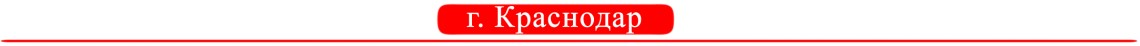
\includegraphics[width=0.7\linewidth]{images/fakt/низ_лого}
% 	\caption{}
% 	\label{fig:}
% \end{figure}
%   % Шапка организации ИП
%%%%%%%%%%%%%%%%%%%%%%%%%%%%%%%%%%%%%%%%%
%
%   Экспертная организация ООО Южнорегиональная экспертная группа
%
%%%%%%%%%%%%%%%%%%%%%%%%%%%%%%%%%%%%%%%%%
\noindent %\qrcode[height=21mm]{\NomerDoc от \окончено }  %%% Добавлен QR-Code
\begin{pspicture}(21mm,21mm)
\obeylines
\psbarcode{%
	%\NomerDoc от \окончено
	BEGIN:VCARD^^J
	VERSION:4.0^^J
	%N:Мраморнов; Александр; Вчеславович^^J
	FN:Александр Мраморнов^^J
%	ORG:IP Alexandr Mramornov^^J
	TITLE: эксперт
	ORG: ИП
	URL:http://www.yourexp.ru^^J
	EMAIL:4516611@gmail.com^^J
	TEL:+7-918-451-6611^^J
	ADR:г. Краснодар, с/т № 2 А/О «Югтекс», ул. Зеленая, 472^^J
	END:VCARD
}{width=1.0 height=1.0}{qrcode}%
\end{pspicture}
\begin{center}
	\normalsize\textbf{$\cdots$\\[-1.5mm] <<$\cdots$>> \\[-5mm]}
	%  
	\noindent\rule{\textwidth}{1pt}\\[-6mm]  % Горизонтальная линия
	% \line(1,0){460}% (1,0) -горизонтальная линия, и (0,1) - вертикальная 
\end{center}

\begin{center}
	\begin{footnotesize}\setstretch{0.3}
		%	\small\textbf\setlength   	%\raisebox{5mm}
		\vspace{-3.5mm}$\cdots$\\[0mm]
		Телефон: \quad $\cdots$, e-mail:\quad $\cdots$\\ [-2mm]{$\cdots$\quad$\cdots$}
	\end{footnotesize}	\\[10mm]
\end{center}


\begin{flushright}
	%Краснодар,
	$\cdots$, 2023    \\[8mm]
\end{flushright}
\begin{center}
	\LARGE\textbf{ ЗАКЛЮЧЕНИЕ ЭКСПЕРТА}
	\bigskip\\[0mm]
	%	{\normnumxtbf{\NomerDoc}}	}{den}
\end{center}
\par
\vspace{-3mm}\noindent по гражданскому делу \delonum \, по иску \isk \\[0mm]

%\raggedright 
%\def\hrf#1{\hbox to#1{\hrulefill}}
\noindent \textbf{№ $\cdots$}\hfill           \textbf{\окончено}\\%[2mm]
%Приостановлено\hfill      \datastop\\
%Возобновлено\hfill          \datarestart\\
%Окончено\hfill                \dataend\\%[4mm]

%\noindent\parbox[l][16mm]{16.5cm}
%{\def\hrf#1{\hbox to#1{\hrulefill}}
%	\noindent Начато\hfill            \datastart\\%[2mm]
%	%	Приостановлено\hfill      \datastop\\
%	%	Возобновлено\hfill          \datarestart\\
%	Окончено\hfill                \окончено\\%[4mm]
%}
%\relax

\begin{flushright}
	\noindent\parbox[l][10 mm]{5cm}
	{\def\hrf#1{\hbox to#1{\hrulefill}}
		\noindent Начато\hfill            \datastart\\%[2mm]
		%	Приостановлено\hfill      \datastop\\
		%	Возобновлено\hfill          \datarestart\\
		Окончено\hfill                \dataend
	}
\end{flushright}
\relax

\datastart г. ~в {\small $\cdots$} \,  при определении  \, \sud  \,  от \, \dataopr \, о назначении \opr \, по гражданскому делу \delonum \, поступили:

\begin{enumerate}\setlist{nolistsep}\item  Материалы гражданского дела \delonum \\[-2mm]
	%	\item  
\end{enumerate}Экспертиза произведена экспертом  $\cdots$
%%%%%%%%%%%%%%%%%%%%%%%%%%%%%%%%%%%%%%%%%%%%%%%%%%

\subsection{Вопросы экспертизы}
\subfile{ask}

\subsection{Исходные данные и объекты исследования}
\subfile{объекты_представленные_на_экспертизу}

\subsection{Заявленные ходатайства}
\subfile{Заявленные_ходатайства}

\subsection{Обстоятельства дела}
\subfile{обстоятельства_дела}

%\subsection{Справочные материалы и нормативные документы}
%\subfile{bib/библиография_суд_ОСАГО}

\printbibliography

\section{Исследование}


\subsection{Термины и определения}
\subfile{термины_определения}

\subsection{Условные обозначения}
\subfile{условные_обозначения}

\subsection{Технические средства}
\subfile{технические_средства}

\subsection{Ограничения по применению исходных данных и предположения, в пределах которых проводилась экспертиза}
\subfile{ограничения}

%%%%%%%%%%%%%%%%  Собственно экспертиза

%\subfile{sections/ОСАГОэкспертизаФакт}
       \subfile{sections/исследованиеОборудования}
%\setcounter{page}{1}
\clubpenalty=10000 
\widowpenalty=10000
\pagestyle{empty} % выключить нумерацию страниц
%%%%%%%%%%%%%%%%%%%%%%%%%%%%%%%%%%%%%%%%%
%
%   Экспертная организация ООО Южнорегиональная экспертная группа
%
%%%%%%%%%%%%%%%%%%%%%%%%%%%%%%%%%%%%%%%%%
\begin{center}
	\normalsize\textbf{ОБЩЕСТВО С ОГРАНИЧЕННОЙ ОТВЕТСТВЕННОСТЬЮ \\[-1.5mm] <<ЮЖНО-РЕГИОНАЛЬНАЯ\quad ЭКСПЕРТНАЯ\quad ГРУППА>> \\[-5mm]}
	%  
	\noindent\rule{\textwidth}{1pt}\\[-6mm]  % Горизонтальная линия
	% \line(1,0){460}% (1,0) -горизонтальная линия, и (0,1) - вертикальная 
\end{center}

\begin{center}
	\begin{footnotesize}\setstretch{0.3}
		%	\small\textbf\setlength   	%\raisebox{5mm}
		\vspace{-3.5mm}350072, Россия, Краснодарский край, г. Краснодар, Ростовское шоссе, 14/2, оф. 67\\[0mm]
		Телефон: \quad 8-918-451-66-11, e-mail:\quad 4516611@gmail.com\\ [-2mm]{ИНН 2311213020\quad КПП 231101001 ОГРН 1162375014560}
	\end{footnotesize}	\\[10mm]
\end{center}





\begin{center}
	\section{{\Large \textbf{ПОРУЧЕНИЕ ЭКСПЕРТУ}}}
\end{center}




В соответствии со ст. 14  ФЗ “О государственной судебно-экспертной деятельности в Российской Федерации“ на основании определения судьи \sud \,  от \dataopr  \, о назначении \opr \, по гражданскому делу \delonum \, по иску \isk \,  директором ООО «Факт»  Юрковой Е.А. производство \opr \, по гражданскому делу \delonum \, поручено эксперту    Мраморнову Александру Вячеславовичу. 






\vspace{30mm}

Директор ООО "ЮРЭГ"\hfill   \rule{4cm}{0.1 mm} \,\,\,  Мраморнов А.В.     
%\setcounter{page}{1}
\clubpenalty=10000 
\widowpenalty=10000
\pagestyle{empty} % выключить нумерацию страниц

%%%%%%%%%%%%%%%%%%%%%%%%%%%%%%%%%%%%%%%%%
%
%   Экспертная организация ООО Южнорегиональная экспертная группа
%
%%%%%%%%%%%%%%%%%%%%%%%%%%%%%%%%%%%%%%%%%
\begin{center}
	\normalsize\textbf{ОБЩЕСТВО С ОГРАНИЧЕННОЙ ОТВЕТСТВЕННОСТЬЮ \\[-1.5mm]<<ЮЖНО-РЕГИОНАЛЬНАЯ\quad ЭКСПЕРТНАЯ\quad ГРУППА>> \\[-5mm]}
	%  
	\noindent\rule{\textwidth}{1pt}\\[-6mm]  % Горизонтальная линия
	% \line(1,0){460}% (1,0) -горизонтальная линия, и (0,1) - вертикальная 
\end{center}

\begin{center}
	\begin{footnotesize}\setstretch{0.3}
		%	\small\textbf\setlength   	%\raisebox{5mm}
		\vspace{-3.5mm}350072, Россия, Краснодарский край, г. Краснодар, Ростовское шоссе, 14/2, оф. 67\\[0mm]
		Телефон: \quad 8-918-451-66-11, e-mail:\quad 4516611@gmail.com\\ [-2mm]{ИНН 2311213020\quad КПП 231101001 ОГРН 1162375014560}
	\end{footnotesize}	\\[10mm]
\end{center}




\begin{center}
	\section{{\Large \textbf{ПОДПИСКА      ЭКСПЕРТА}}}
\end{center}




В соответствии со ст. 14  ФЗ “О государственной судебно-экспертной деятельности в Российской Федерации“ на основании определения судьи \sud \,  от \dataopr  \, о назначении \opr \, по гражданскому делу \delonum \, по иску \isk \,  производство \opr \, по гражданскому делу \delonum \, поручено эксперту   Мраморнову Александру Вячеславовичу. 

\vspace{5mm}

С содержанием ст. 307 УК РФ, предусматривающей уголовную ответственность за дачу заведомо ложного заключения, я, эксперт Мраморнов Александр Вячеславович, ознакомлен.  О  чем и даю настоящую подписку \datastart г.





\vspace{30mm}

{Эксперт}\hfill      \rule{4cm}{0.1 mm} \,\,\,      {Мраморнов А.В.}
%
%%%%%%%%%%%%%%%%%%%%%
%  Блок "Утверждаю"
%%%%%%%%%%%%%%%%%%%%%
\noindent\parbox[l][7cm]{7cm}
{
	 \begin{center}
 \small\textbf{ООО "ЮЖНО-РЕГИОНАЛЬНАЯ ЭКСПЕРТНАЯ ГРУППА"} \centerline{   }
\scriptsize {ИНН 2311213020 КПП 231101001
	 ОГРН 1162375014560}\\
\footnotesize{350072, Россия, Краснодарский край, Ростовское шоссе, 14/2, оф. 67, (861)2-388-399, моб.: 8-918-451-66-11 }
		\end{center}

\hbox to 6cm{\dotfill А.~В.~Мраморнов}}\hfill\parbox[l][7cm]{6cm}
{

 \begin{center}
	\small\textbf{ООО "ЮЖНО-РЕГИОНАЛЬНАЯ ЭКСПЕРТНАЯ ГРУППА"} \centerline{   }
	\scriptsize {ИНН 2311213020 КПП 231101001
		ОГРН 1162375014560}\\
	\footnotesize{350072, Россия, Краснодарский край, Ростовское шоссе, 14/2, оф. 67, (861)2-388-399, моб.: 8-918-451-66-11 }
\end{center}
\hbox to 6cm{\dotfill А.~В.~Мраморнов}}\hfill\parbox[l][7cm]{6cm}


%%%%%%%%%%%%%%%%%%%%%%%%%
% Бок из двух колонок
%%%%%%%%%%%%%%%%%%%%%%%%%
\noindent\parbox[l][5cm]{6cm}{ДФAAL~DKDKDnnnnn-nnnnnnnnnn   mmmmmmmmmmm   mmmmmmmm mmmmmmmmmm mmmmmmmmmmm mmmmmmmm mmmmmmm mmmmmmmmmmm mmmKK FFHHH hdhdhdhhd ррвррввррврврр } \hfill\parbox[l][5cm]{11cm}{ДФAAL DKDKDnnnnnnnnnnnnnnn   mmmmmmmmmmm   mmmmmmmm mmmmmmmmmm mmmmmmmmmmm mmmmmmmm mmmmmmm mmmmmmmmmmm mmmKK FFHHH hdhdhdhhd ррвррввррврврр }

%%%%%%%%%%%%%%%%%%%%%%%%%%%%%%%%
% Пример выделения абзаца с отступом слева
%%%%%%%%%%%%%%%%%%%%%%%%%%%%%%%
\begin{flushleft} 
	\hbox{% 
		\vrule\hspace{.8em}\parbox{1\textwidth}% 
		{Иногда используется следующий способ выделения текста: абзац набирается с некоторым отступом от левого поля, а слева от него, вровень с левым полем, печатается вертикальная линейка.}} 
\end{flushleft}



%%%%%%%%%%%%%%%%%%%  Водяной знак    %%пакет \usepackage{draftwatermark}
%%%%%%%%%%%%%%%%%%%%%%%%%%%

\SetWatermarkLightness{1} % прозрачность
\SetWatermarkText{} % Текст водяного знака
\SetWatermarkScale{0.8}  %масштаб


%%%%%%%%%%%%%%%%%%%%%%%%%%%%%%%%
% Пример два изображения рядом
%%%%%%%%%%%%%%%%%%%%%%%%%%%%%%%
\begin{figure}[h!]\centering
	\parbox[t]{0.49\textwidth}
	{\centering
		\includegraphics[width=.49\textwidth]{example-image}
		\caption{\footnotesize {Этапы реконструкции ДТП}}
		\label{ris:images/1}}
	\hfil \hfil%раздвигаем боксы по горизонтали 
	\parbox[t]{0.49\textwidth}
	{\centering
		\includegraphics[width=.49\textwidth]{example-image}
		\caption{\footnotesize {Этапы реконструкции ДТП}}
		\label{ris:images/39}}
\end{figure}


%%%%%%%%%%%%%%%%%%%%%%%%%%%%%%%%
% Пример изображения рядом подпись к изображению  и само изображение
%%%%%%%%%%%%%%%%%%%%%%%%%%%%%%%

\begin{SCfigure}
	\centering {\footnotesize \caption{Схематичное изображение перераспределения веса автомобиля при торможении  под действием силы $ \vec{F_t}  $ }} 
	\includegraphics[width = 0.6 \textwidth]{example-image}
	\label{ris:images/tormoz}
\end{SCfigure}


%%%%% Текст рядом с изображением


\noindent\begin{minipage}{0.4\linewidth}
    {Величина усилия разрыва болтового соединения известна,
        тогда по правилу отношения плечей приложенных сил: 
        \begin{equation}\label{схемаразрыва}
        \frac{\vec{F_1}}{\vec{F_2}} = \frac{l_2}{l_1}  
        \end{equation}
        $ l_2/l_1 = 470/155 \approx 1/3 $, 
        
        получаем, что для создания усилия разрыва в точке "А", необходимо к точке "В" приложить усилие, равное $\vec{ F_2} = \vec{F_1}/3 = 6 485/3 \approx 2 161 kg $
    }
\end{minipage}
\hfill
\begin{minipage}{0.6\linewidth}
    \begin{center}
        \includegraphics[width=0.9\linewidth]{example-image}
    \end{center}
    \captionof{figure}{Эскиз зуба с расположением разрывных болтов}
\end{minipage}

%%%%%%%%%%%%%%%%%%%%%%%%%%%%%%%%%%%%
%% Два рядом с одной общей подписью 
%%%%%%%%%%%%%%%%%%%%%%%%%%%%%%%%%%%%

\begin{figure}[]
	\begin{minipage}{0.49\textwidth}
		\includegraphics[width=\linewidth]{example-image}
		\subcaption{This is a subfigure}
	\end{minipage}
	\hfill
	\begin{minipage}{0.49\textwidth}
		\includegraphics[width=\linewidth]{example-image}
		\subcaption{This is another subfigure}
	\end{minipage}
	
	\caption{This is a caption for the entire figure}
	\label{fig:twosubs}
\end{figure}



%%%%%%%%%%%%%%%%%%%%%%%%%%%%%%%%%
%  Таблица работ
%%%%%%%%%%%%%%%%%%%%%%%%%%%%%%%%%

\begin{center}
	\begin{tabulary}{\textwidth}{LCL}
		\hline 
		\textbf{Наименование детали}      &   & \textbf{Ремонтное воздействие}\\
		\hline Турбина левая              &   &    Заменить\\
		Блок ДВС                          &   &    Отремонтировать гильзованием, заменой колец и прокладок \\
	\end{tabulary}  
\end{center}


%%%%%%%%%%%%%%%%%%%%%%%%%%%%%%%%%%%%%
% История автомобиля
%%%%%%%%%%%%%%%%%%%%%%%%%%%%%%%%%%%%%
{\small 
	\begin{longtable}{|p{16mm}|p{12mm}|p{29mm}|p{50mm}|p{41mm}|}
		\caption[]{\footnotesize {\textbf{История ремонта и сервисного обслуживания по дате и пробегу}}} \label{tab:hist}\\
		\hline
		%\rowcolor[HTML]{C0C0C0} 
		% Заголовки столбцов
		\textbf{Дата} &\textbf{Пробег, км} &\textbf{№\,Заказ-наряда, накладной}& \textbf{Вид работы}& \textbf{Примечание} \\ \hline \endhead % повторение заголовка 
		% Строки
		22.22.2019 &33\,000  & № 480279303-1 от 03.09.2019& Панель задка  & Замена, окраска \\ \hline
		%\rowcolor[HTML]{EFEFEF} 
		\Rownum & &n & Боковина задняя левая   & Замена, окраска \\ \hline
		%%% ..............& 
	 % Обнуляем счетчик строк для следующей таблицы
	\end{longtable}}
\setcounter{rownum}{0} %сброс счетчика строк в таблице

%%%%%%%%%%%%%%%%%%%%%%%%%%%%%%%%%%%%%%
% Длинная таблица
%%%%%%%%%%%%%%%%%%%%%%%%%%%%%%%%%%%%%%
\begin{longtable}{|p{1cm}|p{11cm}|p{3cm}|}
	\caption[]{\footnotesize {Ремонтные воздействия}} \label{tab:4}\\ 
	\hline
	\rowcolor[HTML]{C0C0C0} 

	\text{N/N} & Наименование запчасти (материала) & Ремонтное воздействие  \\ \hline \endhead % повторение заголовка 
	\Rownum  & Панель задка  & Замена, окраска \\ \hline
	\rowcolor[HTML]{EFEFEF} 
\Rownum  & Боковина задняя левая   & Замена, окраска \\ \hline
	%%% ..............
\end{longtable}

%%%%%%%%%%%%%%%%%%%%%%%%%%%%%%%%%%%%%%%%%%%%%%%
% Таблица аналогов
%%%%%%%%%%%%%%%%%%%%%%%%%%%%%%%%%%%%%%%%%%%%%%%%
\begin{longtable}{|p{5mm}|p{85mm}|p{60mm}|}
	\caption[]{\footnotesize {Описание ТС, идентичных оцениваему}} \label{tab:5}\\ 
	\hline
	\rowcolor[HTML]{C0C0C0} 
	\bf	\text{n/n} &\bf  Описание аналога & \bf URL-адрес преложения  \\ \hline \endhead
	\toprule \centering
	\Rownum  &\includegraphics[width=0.99\linewidth]{example-image} &\noindent {\scriptsize\ https://krasnodar.drom.ru/mazda/mazda6/34943451} \\ \hline 	\centering
	%	\rowcolor[HTML]{EFEFEF} 
	\Rownum  &\includegraphics[width=0.99\linewidth]{example-image} & {\noindent \centering  \scriptsize\ https://krasnodar.drom.ru/mazda/mazda6/34943451} \\ \hline 	\centering
	
\end{longtable}

%%%%%%%%%%%%%%%%%%%%%%%%%%%%%%%%%%%%%%%%
% Таблица длинная по типу таблицы годных остатков
%%%%%%%%%%%%%%%%%%%%%%%%%%%%%%%%%%%%%%%

\begin{longtable}{|p{9cm}|p{4cm}|p{2cm}|}
	\caption[]{\footnotesize {Таблица расчета $ C_i $ }}
	\label{tab:7}\\
	\hline
	Наименование агрегата, узла, детали & \%-ное соотношение (вес)  & Годные, \% \\
	\hline \endhead
	Кузовные детали, экстерьер, интерьер, в т.ч.: & 50 (45 \textless{}1\textgreater{}) & 0 \\
	Передняя часть: & 14 &  \\
	Капот & 1.9 & 1,9 \\
	Крыло переднее (за 1 шт.) & 0.8 & 0,8 \\

	Прочее & 3/8 \textless{}1\textgreater{}/1 \textless{}2\textgreater /6 \textless{}3\textgreater{} & 4 \\
	\hline
	\textbf{ИТОГО,} \%: &  & \textbf{83,8}  \\
	\hline	
\end{longtable}
%%%%%%%%%%%%%%%%%%%%%%%%%%%%%%%%%%%%%%%%%
%%% Таблица с объединением строк 
%%%%%%%%%%%%%%%%%%%%%%%%%%%%%%%%%%%%%%%%%
\begin{table}[H]
	\caption{\label{tab:bolts} Нестандартные болты для левой резьбы.}
	\begin{center}
		\begin{tabular}{|c|c|c|c|c|}
			\hline
			\multirow{3}{*}{Размеры нестандартных болтов} & \multicolumn{2}{c|}{Диаметр} & \multicolumn{2}{c|}{Диаметр2} \\
			\cline{2-5}
			& Норма & Разброс & Норма & Разброс \\
			\cline{2-5}
			& 10 мм & 1 мм & 10 мм & 1 мм \\
			\hline
		\end{tabular}
	\end{center}
\end{table}
%%%%%%%%%%%%%%%%%%%%%%%%%%%%%%%%%%%%%%%%%
%% Таблица с объединение строк и столбцов
%%%%%%%%%%%%%%%%%%%%%%%%%%%%%%%%%%%%%%%%%%

%\begin{table}[ph]
%	\centering
%	\begin{tabular}{c|c|c|c|c}
%		\hline
%		\multirow{2}{*}{Raaa (k)} & \multicolumn{4}{c}{C ()} \\
%		\hline{~----}
%		& 3.3 & 2.5 & 1 & 0.5 \\
%		\hline
%		\multirow{2}{*}{Raaa (k)} & \multicolumn{2}{c|}{\multirow{2}{*}{this}} & 0.5 & 0.6\\
%		\hline{~~~--}            & \multicolumn{2}{c|}{}                      & 0.7 & 1.2 \\
%		\hline
%	\end{tabular}
%	\caption{R, C ripple size}
%	\label{T:peak}
%\end{table}

%%%%%%%%%%%%%%%%%%%%%%%%%%%%%%%%%%%%%%%%%%
%%%%  Таблица повреждений автомобиля
%%%%%%%%%%%%%%%%%%%%%%%%%%%%%%%%%%%%%%%%%%
\begin{longtable}{|M{105mm}|M{50mm}|}
	\caption[]{\footnotesize {Повреждения автомобиля, установленные при его осмотре}} \label{tab:5}\\ 
	\hline
\bf {\small Наименование поврежденной детали с описанием повреждения} & \bf {\small Изображение} \\ \hline \endhead
	%
% {\small    } & \imt{fp1} \\ \hline  % Фото повреждений
	%
{\small Дверь передняя левая -  деформация в труднодоступном месте на площади 6дм2}&  \imt{example-image}\\ \hline 
% {\small    } & \imt{fp1} \\ \hline  % Фото повреждений
% {\small    } & \imt{fp1} \\ \hline  % Фото повреждений
% {\small    } & \imt{fp1} \\ \hline  % Фото повреждений
% {\small    } & \imt{fp1} \\ \hline  % Фото повреждений
% {\small    } & \imt{fp1} \\ \hline  % Фото повреждений
% {\small    } & \imt{fp1} \\ \hline  % Фото повреждений
% {\small    } & \imt{fp1} \\ \hline  % Фото повреждений

\end{longtable}


%%%%%%%%%%%%%%%%%%%%%%%%%%%%%%%%%%%%%%%%%%%%%
%%%%  Таблица ремонтных воздействий
%%%%%%%%%%%%%%%%%%%%%%%%%%%%%%%%%%%%%%%%%%%%%
\begin{longtable}{|p{1cm}|p{11cm}|p{3cm}|}
	\caption[]{\footnotesize {Ремонтные воздействия по акту осмотра № 006/06/19 от \, \osm \, ИП Яковлева С.В.}} \label{tab:4}\\ 
	\hline
	\rowcolor[HTML]{C0C0C0} 
	%	\multicolumn{1}{|c|}
	%	{\cellcolor[HTML]{C0C0C0}N/N} & Наименование запчасти (материала) & Ремонтное воздействие 
	%	
	\text{N/N} & Наименование запчасти (материала) & Ремонтное воздействие  \\ \hline \endhead
	\Rownum  & Панель задка  & Замена, окраска \\ \hline
	\rowcolor[HTML]{EFEFEF} 
	\Rownum  & Боковина задняя левая   & Замена, окраска \\ \hline
	\Rownum  & Боковина задняя правая  & Замена, окраска  \\ \hline
	
\end{longtable}\setcounter{rownum}{0}

%%%%%%%%%%%%  Загрузка данных из csv
                         %%%%%%%%%   CSV    %%%%%%%%%%%%%
\csvautobooklongtable[separator=comma]{csv/test.csv} % semicolon- ;  comma- , pipe- | tab- 	
%%%%%%%%%%%%%%%%%%%%%%%%%%%%%%%%%%%%%%%%%%%%%%%%%%%


%%%%%%%%%%%%%%%%%%%%%% 
%%%  Изображение заданного рамера
%%%%%%%%%%%%%%%%%%%

\includegraphics*[width=5.54in, height=1.66in, keepaspectratio=false]{example-image}
%

%%%%%%%%%%%%%%%%%%%%%%%%%%%%%%%%%%%%%   Сноски %%%%%%%
 \footnote{текст сноски}

%%%%%%%%%%%%%%%%%%%%%%%
%% \usepackage{array} is required
%\begin{tabular}{|>{\raggedright\arraybackslash}p{30mm}|>{\raggedright\arraybackslash}p{95mm}|>{\raggedright\arraybackslash}p{30mm}|}
%	\hline 
%	&  &  \\ 
%	\hline 
%	&  &  \\ 
%	\hline 
%	&  &  \\ 
%	\hline 
%\end{tabular} 
%% \usepackage{array} is required
%\begin{tabular}{|>{\raggedleft\arraybackslash}p{3cm}|>{\raggedleft\arraybackslash}p{3cm}|>{\raggedleft\arraybackslash}p{3cm}|}
%	\hline 
%	&  &  \\ 
%	\hline 
%	&  &  \\ 
%	\hline 
%\end{tabular} 
%% \usepackage{array} is required
%\begin{tabular}{|>{\raggedright\arraybackslash}p{3cm}|>{\centering\arraybackslash}p{%<3cm%>}|>{\centering\arraybackslash}p{%<3cm%>}|}
%			\hline 
%			&  &  \\ 
%			\hline 
%			&  &  \\ 
%			\hline 
%		\end{tabular} 
%		
%		
%%%%%%%%%%%%%%%% ПРОСТАЯ ТАБЛИЦА ПОВРЕЖДЕНИЙ
%
%{\small \begin{table}[]
%\begin{longtable}{@{}ll@{}}
%	\caption[]{\footnotesize {\textbf{Описание повреждений деталей}}} \label{tab:4}\\ 
%		\toprule
%	\textbf{	Наименование детали       }               &\textbf{ Описание повреждений}                         \\ \midrule
%		Решетка бампера переднего средняя        & разбита                                      \\
%		Решетка бампера левая                    & оборваны, деформированы крепежные кронштейны \\
%		%.................................
%		Заднее правое крыло                      & несложная деформация, повреждение ЛКП        \\ \bottomrule
%	\end{longtable}
%\end{table}}

%%%%%%%%%%%%%%%%% ПРОСТАЯ ТАБЛИЦА РЕМОНТНЫХ ВОЗДЕЙСТВИЙ

{\small \begin{table}
	\begin{longtable}{@{}ll@{}}
	\caption[]{\footnotesize {\textbf{Назначенные ремонтные воздействия}}} \label{tab:2}\\ 
	\toprule
\textbf{Наименование детали}                      & \textbf{Ремонтные воздействия}\\ \midrule
Решетка бампера переднего средняя        & заменить             \\
%......................
Заднее правое крыло                      & ремонт 3 ч, окрасить \\ \bottomrule
\end{longtable}

\end{table}}


%%%%%%%%%%%%%%%%%%%%%%%%%%%%%%%%%%%
%%%
%%% ТАБЛИЦА  ДЛИННАЯ ТОНОВАЯ РАЗМЕТКА
%%%%%%%%%%%%%%%%%%%%%%%%%%%%%%%%%%%
 \begin{table}[H]
 	\centering
  	\caption{{\footnotesize Запчасти и материалы к заказ-наряду № Ш000011955 от 10.08.2017}}
 	\label{tab:4}
 	\begin{tabular}{|l|ll|l|l|}
 		\hline
 		\rowcolor[HTML]{C0C0C0} 
 		\multicolumn{1}{|c|}{\cellcolor[HTML]{C0C0C0}N кат} & Наименование запчасти (материала) & & Цена за шт. & Всего цена, руб \\ \hline
		7109113821    & Хомут пластиковый самозатяжной  & & 5      & 50      \\ \hline
	    \rowcolor[HTML]{EFEFEF} 
		0411151042    & Ремкомплект ДВС 1VDFTV (1 шт.)      & & 16000     & 16000    \\ \hline
		1111551030С0    & Прогкладка ГБЦ правая  (1 шт.)    & & 3250     & 3250      \\ \hline
		\rowcolor[HTML]{EFEFEF} 
		1111651030С0    & Прокладка ГБЦ левая (1 шт.) & & 3250     & 3250      \\ \hline
		131010W011B0    & Поршень левый (4 цил)      & & 4900     & 19600      \\ \hline
		\rowcolor[HTML]{EFEFEF} 
		131010W021B0   & Поршень правый (4 цил.)  & & 5000     & 20000      \\ \hline
		1301151040    & Кольца поршневые комплект (8цил)      & & 38     & 49000      \\ \hline
%%%  ........................
			\rowcolor[HTML]{EFEFEF} 
 		103223   & Масло трансмиссионное Multi ATF (1.3 л)     & & 750   & 975      \\ \hline
 	%	17   & Клапан (16 шт.)       & 1150     & 18400      \\ \hline& 
 		\end{tabular}
\end{table}

\end{document} 
